\part{Estimation of Hawkes' parameters}
\chapter{Introduction to Estimation}

This part investigates the problem of recovering information about data generated by Hawkes processes given by a set of parameters $\Theta = ( \nu, \alpha, \beta ) $, and for which we observe a set of jumps' times. The process can be multivariate, and we would like:

\begin{itemize}
\item to estimate the parameters $\theta$ by $\hat{\theta} = ( \hat{\nu}, \hat{\alpha}, \hat{\beta} )$. $\theta$ shall belong to a set of possible parameters, named $\Theta$.

\item to estimate the parameters with some temporal dependency on them. We then replace our estimate by: $\hat{\theta}_t$,
\item to analyze the evolution of parameters on the angle of change point analysis, and we could try to incorporate that analysis inside our estimation process, in an attempt to increase the accuracy of our estimation.
\end{itemize}


The estimators are tested over simulated data, for the sake of simplicity and lack of relevant data. Unfortunately, this method bypasses the many significant challenges raised by real datasets, challenges that caused \cite{critic_hawkes} to state that:

\textit{"Our overall conclusion is that calibrating the Hawkes process is akin to an excursion within a minefield that requires expert and careful testing before any conclusive step can be taken."}

The method considered is maximum likelihood estimation, which begins by finding the likelihood function, and estimates the model parameters as the inputs which maximise this function.

Recall that the observed information is lying in the time-interval $[0,T]$.
\chapter{Estimation : a First Approach}

\section{Introduction to Max. Likelihood Estim. (MLE)}

The Maximum Likelihood Estimator (MLE) is commonly used in order to find an estimator of the parameters. However, it has been a challenge for quite a long time, quoting \cite{daley}:

\textit{The likelihood functions for most of the processes discussed [...] are relatively intractable. This difficulty was a block to the application of general point process models until the late 1960s, when a quite different approach was introduced in papers on filtering theory pioneered by the electrical engineers. [...] Once recognised, its role in elucidating the structure of point process likelihoods was soon exploited. General definitions of the conditional intensity function were given in Rubin (1972) and especially by Brémaud (1972), in whose work conditional intensity functions were rigorously defined and applied to likelihood and other problems (see also Brémaud, 1981).}

Optimization theory (for finding maximums) is very dense, and since the log-likelihood of Hawkes processes is non-linear, we would like to use a non-linear optimization technique. 

Ozaki in \cite{Ozaki} in section 3 mentions three methods for finding the maximum likelihood

\begin{itemize}
\item Gradient and Hessian (Newton-Raphson method)
\item Gradient (Davidon's procedure)
\item only the likelihood function (direct method)
\end{itemize}


We are going to use the Newton-Raphson method. Though it might be more expensive to compute the Hessian, it leads to better estimators.


For that purpose, we need to compute numerically the gradient and the hessian of the log-likelihood. One can find their expressions in the univariate case in Ozaki's paper (\cite{Ozaki}) but the author couldn't find any paper on the multivariate case. For that reason, we computed the algebraic expressions by hand, before putting them into code. One has to be quite careful about the code since the derivatives are very expensive to compute. We give a list of advice at the end of the chapter.





\subsection{Derivation of the Likelihood Function}
\begin{theoreme}{Likelihood of a simple point process}
From definition 7.1.II in \cite{daley}; let us say that a simple point process has list-history: $\sequence{ t_i }$, on a bounded Borel set $A$. Then, the likelihood of a process $N$ can be expressed as:
\begin{equation}
L( \theta \mid \sequence{t_i} ) =  \frac{\mathbb P \left (N_{\theta}  \text{ has } \# \sequence{t_i} \text{ points in } A \text{ at locations  } (d t_1, \cdots, d t_n) \right ) } {(d t_1, \cdots, d t_n)}
\end{equation}

Notice that since $A$ is bounded, the sequence is finite so the $\#\sequence{t_i}$ number of elements is finite too. 
\end{theoreme}




In order to have a closed form expressions for the term $$\frac{\mathbb P \left (N_{\theta}  \text{ has } \# \sequence{t_i} \text{ points in } A \text{ at locations  } (d t_1, \cdots, d t_n) \right ) } {(d t_1, \cdots, d t_n)}  =: \mathbb P ( \mathcal N_{\theta} ) $$

we introduce a function:
\begin{definition}[Conditional Survivor Functions]
\begin{equation}
\forall u \in \R, k \in \N, \qquad S_k ( u \mid t_1, \cdots, t_{k-1} ) = \mathbb P ( t_k - t_{k-1} > u \mid t_1, \cdots, t_{k-1} ) 
\end{equation}
\end{definition}



Then, one can actually prove that for every simple point process, there exists a unique family of survivor functions such that

\begin{theoreme}{Associated Survivor to a Simple Point Process}
From proposition 7.2.I in \cite{daley}; we have that there exists a unique family of conditional probability density functions $\sequence{p_i}$\footnote{Thus there exists a bijection between the families of probability density functions as described and the marked point process.} and associated survivor functions, related in the following way:
\begin{equation}
\forall 0 < t_1 < \cdots < t_{n-1} < t, \quad S_n( t \mid t_1, \cdots, t_{n-1} ) = 1 - \int_{t_{n-1}}^t p_n ( u \mid t_1, \cdots, t_{n-1} ) du
\end{equation}
Then, we have the following expression whenever $0 < t_1 < \cdots < t_{n} < T < \infty $:
\begin{equation}
\mathbb P ( \mathcal N_{\theta} )  =   \prod_{i = 1}^n p_i ( t_i \mid t_1 \cdots t_{i-1} ) \times S_{n+1} ( T \mid t_1, \cdots, t_n )  
\end{equation}
\end{theoreme}


\begin{remarque}
In layman terms, $p_n$ is the conditional probability density function of the time of the next event knowing the previous events
\end{remarque}


\begin{theoreme}[label = theoreme_expression_ln_lik]{Closed Form of the Likelihood for a Simple Point Process}
If $N$ is a simple point process on $[0,T]$,  $0 < T < \infty$, and we are aware of the realization of $N$ over $[0,T]$ as being $\sequence{t_i}$, then the likelihood $L$ of $N$ reads:
\begin{align}
L( \theta \mid \mathcal F ) &= \exp \left ( - \int_{0}^{T} \lambda_{\theta} ( s \mid \mathcal F ) ds \right )  \prod_{i=1}^{N(T)}  \lambda_{\theta} ( T_i = t_i \mid \mathcal F_{t_{i-1}^-} )  
\end{align}
\end{theoreme}


\begin{demo}{}{}
Let us assume that $N(T) = \# \sequence{ t_i } =: n$.

Given in definition \ref{def:lambda_1}, we have:
$$\lambda_{\theta}( T_n = t \mid \mathcal F_{t^-} ) = \frac{ p_n( t \mid \mathcal F_{t^-} )}{S_n( t \mid \mathcal F_{t^-} )}$$


yielding  this rough idea of inversion:

\begin{align*}
\forall i \leq n, \quad \int_{t_i}^t \lambda_{\theta}( T_i = s \mid \mathcal F_{s^-} ) ds &= - \ln ( S_i (t \mid \mathcal F_{t^-} ))  \\
& \iff \\
\forall i \leq n, \quad  S_i( t \mid \mathcal F_{t^-} ) & = 1 -  \exp \left ( - \int_{t_i}^t \lambda_{\theta} ( s \mid \mathcal F_{s^-} ) \right ) ds \\
& \qquad \text{ and } \\
\forall i \leq n, \quad  p_i( T_i = t \mid \mathcal F_{t^-} ) & = \lambda_{\theta} ( T_i = t \mid \mathcal F_{t^-} ) \\
& \times \quad \exp \left ( - \int_{t_i}^t \lambda_{\theta} ( s \mid \mathcal F_{s^-} ) \right ) ds 
\end{align*} 


We get that the likelihood can be written as:
\begin{align}
L( \theta \mid \mathcal F ) &= \prod_{i=1}^n p_i( T_i = t_i \mid \mathcal F_{t_{i-1}} ) \times S_{n+1} ( T \mid t_1, \cdots, t_n ) \notag \\
&=  \prod_{i=1}^n  \lambda_{\theta} ( T_i = t_i \mid \mathcal F_{t_i^-} ) \exp \left ( - \int_{t_{i-1}}^{t_{i}} \lambda_{\theta} ( s \mid \mathcal F_{t_i} ) ds \right ) \notag \\
 & \qquad \times \exp \left ( - \int_{t_n}^T \lambda_{\theta} ( s \mid \mathcal F_{t_n} ) ds \right ) \notag \\
&=  \exp \left ( - \int_{0}^{T} \lambda_{\theta} ( s \mid \mathcal F ) ds \right )  \prod_{i=1}^n  \lambda_{\theta} ( T_i = t_i \mid \mathcal F_{t_{i-1}^-} )   
\end{align}
\end{demo}{}{}













\subsection{Theory of MLE}
We derived an expression for the likelihood in the previous subsection (recall theorem \ref{theoreme_expression_ln_lik}). 

Directly, we derive the log-likelihood of a simple point process, for which one knows the conditional intensity function $\lambda$. It reads:

\begin{align}
\ln L( \theta \mid \Tau, \lambda ) &= - \int_0^T  \lambda(s \mid \mathcal F_{s^-}) ds + \int_0^T  \ln \lambda(s \mid \mathcal F_{s^-} )d N_s \notag \\
&=  - \int_0^T \lambda(s \mid \mathcal F_{s^-}) ds + \int_0^T  \ln \lambda(s \mid \mathcal F_{s^-} )d N_s 
\label{eq:intensity_lambda}
\end{align}

We highlight the presence of the integral of the conditional intensity function over time, which is known as the compensator of the point process, relative to some given history $\mathcal F$. 


\begin{definition}[Compensator]
\label{def:compensator}
For a counting process $N$ we define the function $$\Lambda(t) = \int_0^t \lambda (s \mid \mathcal F_{s^-} ) ds $$  to be the compensator of the counting process.
\end{definition}

That quantity has actually some meaningful properties,

\begin{theoreme}{Compensator as the Drift Part of a Martingale}
Assume that N is $\mathcal F$-adapted and admits a left-continuous conditional intensity $\lambda$. Then the process $M(t) = N(t) - \Lambda (t)$ is a $\mathcal F$ martingale, i.e.:

$$\forall 0 < t < s, \E [ M(s) \mid \mathcal F_t ] = M(t)$$
\end{theoreme}


\begin{demo}{}{}
Some intuition behind that theorem is given in \cite{daley}.

Intuitively, $\E[M(s) \mid \mathcal F_t]$ is constant because, for a small increment $\Delta$:

\begin{align*}
\E \left [ M( t + \Delta ) - M(t) \right ] &= \E \left[ N(t+ \Delta ) - N(t) - \Lambda( t + \Delta) + \Lambda(t) \mid \mathcal F_t \right ] \\
&\approx   \E \left[ N(t+ \Delta ) - N(t) \mid \mathcal F_t \right ] - \lambda(t) \Delta  \\
&\approx \left ( \lambda(t) - \lambda(t) \right  ) \Delta  \\
&= 0 
\end{align*}
In other words, the compensator is centring the counting process around zero: 

$$\E [ N^m (t) - N^m (0) ] = \E  \left  [ \E [ N^m (t) - N^m (0) \mid \Lambda_m(t) ]  \right ] = \E [ \Lambda_m (t) ] $$

\end{demo}

Actually, the decomposition of the process into the compensator and a martingale comes from the Doob-Mayer decomposition. A very common technique when looking at general stochastic processes is to break them down into separate martingale and drift terms. 

This is easiest to describe in the discrete time situation. So, suppose that the process $\sequence{X_i}$  is a stochastic process adapted to the discrete-time filtered probability space  $(\Omega, \mathcal F, \mathcal F_n, \mathbb P )$. If $X$ is integrable, then it is possible to decompose it into the sum of a martingale $M$ and a process $\Lambda$, starting from zero, and such that $\Lambda_n$ is $\mathcal{F}_{n-1}$-measurable for each $n\ge1$. That is, $\Lambda$ is a predictable process. The martingale condition on $M$ enforces the identity:

\begin{equation}
\Lambda_n-\Lambda_{n-1}={\mathbb E}[\Lambda_n-\Lambda_{n-1}\vert\mathcal{F}_{n-1}]={\mathbb E}[X_n-X_{n-1}\vert\mathcal{F}_{n-1}]
\end{equation}

So, $\Lambda$ is uniquely defined by
\begin{equation}
\Lambda_n=\sum_{k=1}^n{\mathbb E}\left[X_k-X_{k-1}\vert\mathcal{F}_{k-1}\right]
\end{equation}

and is referred to as the compensator of $X$. Essentially, it is the predictable term in the Doob decomposition.


In continuous time, where we work with respect to a complete, as well as, filtered probability space $(\Omega,\mathcal{F},\{\mathcal{F}_t\}_{t\ge0},{\mathbb P})$, the situation is much more complicated. There is no simple explicit formula for the compensator of a process. Instead, it is defined as follows.

Under regularity condition of the adapted process (finite variation and cadlag), the compensator $\Lambda $ is defined with $\Lambda_0=0$, such that $X-\Lambda$ is a local martingale. 


\begin{theoreme}{Existence of compensator}
The processes for which a compensator exists are precisely the special semimartingales or, equivalently, the locally integrable semimartingales. 
\end{theoreme}

In particular, all continuous and adapted processes are predictable but, due to the existence of continuous martingales such as Brownian motion, this means that decompositions as sums of martingales and predictable processes are not unique. It is therefore necessary to impose further conditions on the term $\Lambda$ in the decomposition. It turns out that we obtain unique decompositions if, in addition to being predictable, $\Lambda$ is required to be cadlag with locally finite variation. 

One can prove that both definition (Doob-Meyer decomposition and definition \ref{def:compensator}) agree.

Recall from eq. (\ref{eq:stieltjes_integral3}), the conditional intensity for a $M$-multivariate Hawkes process reads:

\begin{align}
\lambda^{m} (t \mid \Tau_{t^-} ) &= 
\nu_m + \sum_{n = 1}^M \sum_{ \{k: t_k^n < t \}} \alpha_{m,n} e^{- \beta_{m,n} \cdot ( t - t_k^n ) } 
\end{align}


Then we can write the compensator for a multivariate Hawkes process as:

\begin{align}
\Lambda^{m}(T) &= - \int_0^T \left [ \nu_m + \sum_{n = 1}^M \sum_{ \{k: t_k^n < t \}} \alpha_{m,n} e^{- \beta_{m,n} \cdot ( t - t_k^n ) } \right ] dt \notag \\
&=  - \int_0^T \nu_m dt  + \sum_{n = 1}^M  \int_0^T \sum_{ \{k: t_k^n < t \}} \alpha_{m,n} e^{- \beta_{m,n} \cdot ( t - t_k^n ) } dt
\label{eq:compensator}
\end{align}

which, when the parameters are constant with respect to time, reduces to:

\begin{align}
\Lambda^{m}(T) = - \nu_m T  - \sum_{n = 1}^M  \frac{\alpha_{m,n}}{ \beta_{m,n} } \sum_{ \{k: t_k^n < T \}} \left ( 1 - e^{- \beta_{m,n} \cdot ( T - t_k^n ) }  \right ) 
\label{eq:compensator_constant}
\end{align}

We then use the expression of the conditional intensity and the compensator inside the log-likelihood, i.e. equations (\ref{eq:stieltjes_integral3}) and (\ref{eq:compensator}) inside (eq. \ref{eq:intensity_lambda}). We get:


\begin{align}
\ln L( \theta \mid \Tau, \lambda^{m} ) &=  T - \int_0^T \lambda^m(t \mid \mathcal F_{t^-}) ds + \int_0^T  \ln \lambda^{m}(t \mid \mathcal F_{t^-} )d N_t  \notag \\
&= T - \Lambda^{m}(T) + \sum_{i=1}^n  \ln \lambda^{m}(t_i \mid \mathcal F_{t_i^-} ) \notag \\
&= 
T - \int_0^T \nu_m dt  + \sum_{n = 1}^M  \int_0^T \sum_{ \{k: t_k^n < t \}}  \alpha_{m,n} e^{- \beta_{m,n} \cdot ( t - t_k^n ) } dt \notag
\\ &  \qquad + \sum_{i=1}^n  \ln \left ( 
\nu_m + \sum_{n = 1}^M \sum_{ \{k: t_k^n < T \}} \alpha_{m,n} e^{- \beta_{m,n} \cdot ( T - t_k^n ) }
\right ) 
\end{align}

which in the case of constant parameters, reduces to:

\begin{theoreme}[label = thrm:ln-like]{Log Likelihood: $M$-variate Hawkes with constant parameters}
\begin{align}
\ln L( \theta \mid \Tau, \lambda^{m} ) &= - \nu_m T  - \sum_{n = 1}^M \frac{\alpha_{m,n}}{ \beta_{m,n} } \sum_{ \{k: t_k^n < T \}} \left ( 1 - e^{- \beta_{m,n} \cdot ( T - t_k^n ) }  \right )  \notag
\\ & \quad \qquad + \sum_{i=1}^n  \ln \left ( 
\nu_m + \sum_{n = 1}^M \sum_{ \{k: t_k^n < T \}} \alpha_{m,n} e^{- \beta_{m,n} \cdot ( T - t_k^n ) }
\right ) 
\end{align}
\end{theoreme}







\section{Algorithm for Estimation}
With the expression of the likelihood for a Hawkes Process, it is now possible to find the MLE. We use a classic multivariate Newton-Raphson algorithm. 

\subsection{Multivariate Newton Raphson Algorithm}
For the sake of completeness, we include the basic idea behind a multivariate Newton Raphson algorithm. 


\willdo{ i have that to write} 

\begin{theoreme}{Step of the Multivariate Newton Raphson Algorithm}
One iteration of the algorithm corresponds to do...
\end{theoreme}

\subsection{Implementation and Optimization}
It can be quite challenging to use this algorithm for Hawkes Processes. First, there is a computational bottleneck due to the computation of the expressions of $R, R', R''$, defined in subsection \ref{subsection_R_def} and that appears in the computations of the log-likelihood. There is unfortunately, up-to-now, no recursive formulas for $R'$ and $R''$. 

We show the mean time required for simulating and applying the Newton-Raphson algorithm to one process, while changing the number of jumps of the process. The fig. \ref{fig:complex} displays a quadratic tendency. The usage of the profiler shows that most of the computations come from the bottleneck.  

\begin{figure}
\centering
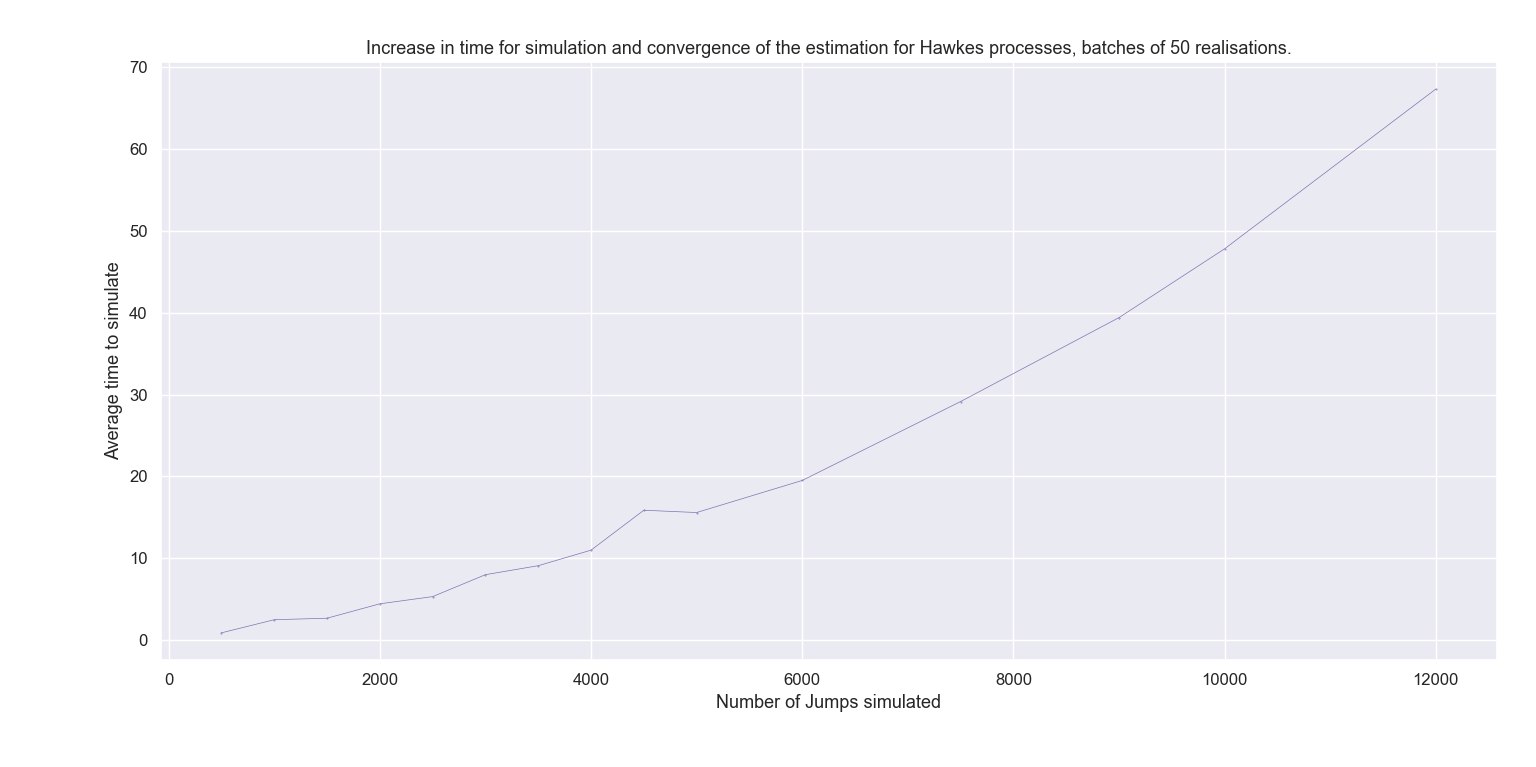
\includegraphics[width = 0.90 \textwidth]{../imag/chap2/complexity.png}
\caption{Time in seconds in order to simulate and estimate one Hawkes Process. The plot shows a quadratic trend for the complexity.}
\label{fig:complex}
\end{figure}

Another issue while using the Newton-Raphson is the neither regular nor convex nature of the derivatives. This leads to the existence of numerous local maxima of the log-likelihood. Hence, the result of an estimation might be a local maxima instead of the desired global maxima. For that reason, a usual technique for checking is using a few different initial conditions or using another searching method.















\section{Numerical Required Computations}
\subsection{Gradient and Hessian's values}
\label{subsection_R_def}

We found out in theorem \ref{thrm:ln-like} that the log-likelihood of a Hawkes process with exponential decay has a closed form. What about the multivariate likelihood?

\vspace{0.6 cm}
\underline{\textbf{Likelihood Function}}

Likelihood function of the multivariate Hawkes process is given by:

\begin{equation}
\ln L( \theta \mid \Tau ) = \sum_{m = 1}^M \ln L^m( \theta \mid \Tau )
\label{eq:ln_multi}
\end{equation}

This follows from the previous theorem \ref{thrm:ln-like}. A more detailed explanation is given in \cite{Likelihood_Hawkes}.



We fix $m,n$ as being inside $\llbracket 1, M \rrbracket ^2 $. Also notice that the $m$-th likelihood is only influenced by a subset of the parameters:

\begin{align*}
\forall m \in \llbracket 1, M \rrbracket , \  \ln L^m( \theta \mid \Tau ) &= \ln L^m( 
\{ \nu_i \}_{ i \in  \llbracket 1, M \rrbracket  },
\{ \alpha_{i,j} \} _{ i,j \in  \llbracket 1, M \rrbracket ^2 },
\{ \beta_{i,j} \}_{ i,j \in  \llbracket 1, M \rrbracket ^2 }
\mid \Tau ) \\
&= \ln L^m( 
\{ \nu_m \},
\{ \alpha_{m,j} \} _{ j \in  \llbracket 1, M \rrbracket  },
\{ \beta_{m,j} \}_{j \in  \llbracket 1, M \rrbracket  }
\mid \Tau )
\end{align*}

In other words, the gradient simplifies to its corresponding marginal gradient. 

Then, we introduce the function $R$ inside theorem \ref{thrm:ln-like}. The log-likelihood reads:


\begin{align}
\ln L^m( \theta \mid \Tau ) = - \nu_m T &- \sum^p_{n=1} \frac {\alpha_{m,n} } {\beta_{m,n}}  \lsum{n} (1 - \lexp{n}) \notag \\ 
&+ \lsum{m} \ln \left ( \denomR \right ) 
\end{align}

where $R_{m,n}$ is defined as $R_{m,n}(1) = 0 $ and for $k \geq 1$ as  

\begin{equation*}
\forall k \geq 2, \qquad R_{m,n} (k) = \sum_{ \{i : t_i^n < t_k^m \} } \exp \left ( - \beta_{m,n} \cdot ( t_k^m - t_i^n )  \right ) 
\end{equation*}

We will prefer, instead of it, this recurrent expression which leads to faster computations:

\begin{align*}
k = 1, \quad R_{m,n} (k) &= 0 \\
k \geq 2, \quad R_{m,n} (k) &= \exp ( - \beta_{m,n} \cdot ( t_k^m - t^m_{k-1} ) ) R_{m,n} (k-1) \\ 
& + \sum_{ \{i: t_i^n \in [ \ t_{k-1}^m, t_k^m \ [ \  \} } \exp ( - \beta_{m,n} ( t^m_k - t_i^n ) )
\end{align*}


\begin{remarque}
Notice that it is possible to use this less expensive expression in the case $m=n$: 
$$k \geq 2, \quad R_{m,n} (k) = \exp ( - \beta_{m,n} \cdot ( t_k^m - t^m_{k-1} ) ) (1 + R_{m,n} (k-1))$$

\end{remarque}

Furthermore, we will also need the derivatives of those expression for which no useful recurrent expression exists yet. 


\begin{align*}
k = 1, \quad R'_{m,n} (k) &= 0 \\
k \geq 2, \quad R'_{m,n} (k) &= \sum_{ \{i : t_i^n < t_k^m \} } (t_k^m - t_i^n)  \exp \left ( - \beta_{m,n} \cdot ( t_k^m - t_i^n ) \right )
\end{align*}


\begin{align*}
k = 1, \quad R''_{m,n} (k) &= 0 \\
k \geq 2, \quad R''_{m,n} (k) &= \sum_{i : t_i^n < t_k^m } (t_k^m - t_i^n)^2  \exp ( - \beta_{m,n} \cdot ( t_k^m - t_i^n ) )
\end{align*}















\vspace{0.6 cm}
\underline{\textbf{First order derivatives}}
\begin{equation}
\frac{\partial } {\partial \nu_m} \ln L^m ( \theta \mid \Tau ) = - T + \lsum{m} \frac 1 {\denomR}
\end{equation}
\begin{align}
\frac{\partial  } {\partial \alpha_{m,n}} \ln L^m ( \theta \mid \Tau ) &= - \frac 1 {\beta_{m,n}} \lsum{n} ( 1 - \lexp{n} ) \notag \\ &+ \lsum{m} \frac{R_{m,n}(k)}{\denomR}
\end{align}

\begin{align}
\frac{\partial  } {\partial \beta_{m,n}} \ln L^m ( \theta \mid \Tau ) &= \frac {\alpha_{m,n}} {\beta_{m,n}^2} \lsum{n} ( 1 - \lexp{n} ) \notag \\ 
&-  \frac{ \alpha_{m,n} } { \beta_{m,n} } \lsum{n} ( T-t_k^n) \lexp{n} ) \notag \\ 
&- \lsum{m} \frac{\alpha_{m,n} R'_{m,n} (k) }{ \denomR}
\end{align}















\vspace{0.6 cm}
\underline{\textbf{Second order derivatives}}

\begin{equation}
\frac{\partial^2  } {\partial \nu_m^2} \ln L^m ( \theta \mid \Tau ) = -  \lsum{m} \frac 1 { \left (\denomR \right )^2}
\end{equation}
\begin{equation}
\frac{\partial^2 } {\partial \nu_m \partial \nu_{m'}} \ln L^m ( \theta \mid \Tau ) = 0, \qquad m \neq m'
\end{equation}


\begin{equation}
\frac{\partial^2  } {\partial \alpha_{m,n}^2} \ln L^m ( \theta \mid \Tau ) = - \lsum{m} \left [ \frac{R_{m,n}(k)}{\denomR} \right ] ^2
\end{equation}
\begin{equation}
\frac{\partial^2 } {\partial \alpha_{m,n} \partial \alpha_{m,n'} } \ln L^m ( \theta \mid \Tau ) =  - \lsum{m}  \frac{R_{m,n}(k) R_{m,n'}(k) }
{\left ( \denomR  \right ) ^2}, \qquad n \neq n'
\end{equation}
\begin{equation}
\frac{\partial^2 } {\partial \alpha_{m,n} \partial \alpha_{m',n'} } \ln L^m ( \theta \mid \Tau ) = 0 , \qquad m \neq m'; n,n' \in  \llbracket 1, M \rrbracket
\end{equation}

\begin{equation}
\frac{\partial^2 } {\partial \nu_m \partial \alpha_{m,n} } \ln L^m ( \theta \mid \Tau ) =  - \lsum{m}  \frac{R_{m,n}(k) }{  \left ( \denomR \right )^2} 
\end{equation}

\begin{equation}
\frac{\partial^2  } {\partial \nu_m \partial \alpha_{m',n} } \ln L^m ( \theta \mid \Tau ) = 0 , \qquad m \neq m', n \in  \llbracket 1, M \rrbracket
\end{equation}



\begin{align}
\frac{\partial^2 } {\partial \beta_{m,n}^2} \ln L^m ( \theta \mid \Tau ) = & - 2 \frac {\alpha_{m,n}} {\beta_{m,n}^3} \lsum{n} ( 1 - \lexp{n} ) \notag \\ 
+  2 \frac{ \alpha_{m,n} } { \beta_{m,n}^2 } & \lsum{n} ( T-t_k^n) \lexp{n} )  \notag \\
+ \frac{ \alpha_{m,n} } { \beta_{m,n} } & \lsum{n} ( T-t_k^n)^2 \lexp{n} )  \notag \\ 
+ \lsum{m} & \left (  \frac{\alpha_{m,n} R''_{m,n} (k) }{ \left ( \denomR \right )^2} - \left ( \frac{\alpha_{m,n} R'_{m,n} (k) }{ \denomR} \right )^2 \right ) 
\end{align}

\begin{equation}
\frac{\partial^2 } {\partial \beta_{m,n} \partial \beta_{m,n'} } \ln L^m ( \theta \mid \Tau ) =  - \lsum{m} \frac{\alpha_{m,n} R'_{m,n}(k) \alpha_{m,n'} R'_{m,n'}(k) }{ \left ( \denomR \right )^2}, \qquad n\neq n'
\end{equation}

\begin{equation}
\frac{\partial^2 } {\partial \beta_{m,n} \partial \beta_{m',n'} } \ln L^m ( \theta \mid \Tau ) = 0, \qquad m \neq m'; n,n' \in  \llbracket 1, M \rrbracket
\end{equation}



\begin{equation}
\frac{\partial^2 } {\partial \nu_m \partial \beta_{m,n} } \ln L^m ( \theta \mid \Tau ) = \lsum{m} \frac{\alpha_{m,n} R'_{m,n}(k)}{\left ( \denomR \right )^2}
\end{equation}

\begin{equation}
\frac{\partial^2 } {\partial \nu_m \partial \beta_{m',n} } \ln L^m ( \theta \mid \Tau ) = 0, \qquad m \neq m'; n \in  \llbracket 1, M \rrbracket
\end{equation}


\begin{align}
\frac{\partial^2 } { \partial \beta_{m,n} \partial \alpha_{m,n} }  \ln L^m ( \theta \mid \Tau ) =  & \frac {1} {\beta_{m,n}^2} \lsum{n} ( 1 - \lexp{n} ) \notag \\ 
&-  \frac{ 1 } { \beta_{m,n} } \lsum{n} ( T-t_k^n) \lexp{n} ) \notag \\ 
&- \lsum{m} \frac{ R'_{m,n} (k) }{ \denomR  } \notag \\
&+ \lsum{m} \frac{ \alpha_{m,n} R'_{m,n} (k) R_{m,n}(k) }{ \left ( \denomR \right )^2 }
\end{align}

\begin{equation}
\frac{\partial^2 } { \partial \beta_{m,n} \partial \alpha_{m,n'} } \ln L^m ( \theta \mid \Tau ) = \lsum{m} \frac{ \alpha_{m,n} R'_{m,n} (k) R_{m,n'}(k) }{ \left ( \denomR \right )^2 }, \qquad n \neq n'
\end{equation}

\begin{equation}
\frac{\partial^2 } {\partial \alpha_{m,n} \partial \beta_{m',n'} } \ln L^m ( \theta \mid \Tau ) = 0, \qquad m \neq m'; n,n' \in  \llbracket 1, M \rrbracket
\end{equation}
